\section{Experiments}\label{sec:trf:experiments}

In this section we apply the techniques in this chapter to realistic datasets of molecular fingerprints.
All experiments were performed in python using the
\texttt{numpy} \citep{harris2020array},
\texttt{pytorch} \citep{paszke2019pytorch},
\texttt{gpytorch} \citep{gardner2018gpytorch},
and \texttt{rdkit} \citep{rdkit-version-2023-09-01} packages.
Molecules were represented with both binary (B) and count (C) Morgan fingerprints
of dimension 1024 (introduced in \S\ref{sec:background:fingerprints}).\footnote{
    Note that when using count fingerprints for $T_{DP}$ post-processed each vector to contain
    the \emph{square root} of the counts of each subgraph.
    This was done for two reasons:
    \begin{enumerate}
        \item To reduce the norms of the vectors (and thereby increase $\zeta$).
        \item To roughly make their interpretation consistent with $T_{MM}$: i.e.\@ the ``weight'' of a fragment in which occurs $n$ times in the numerator/denominator of $T_{DP}$ is $n$ times the weight of a fragment which occurs once.
    \end{enumerate}
}
Code to reproduce all experiments is available at: \TRFcodeURL{}.

\subsection{Errors of random features on real datasets}\label{sec:expt-rf-on-real-data}

\begin{figure}
    \centering
    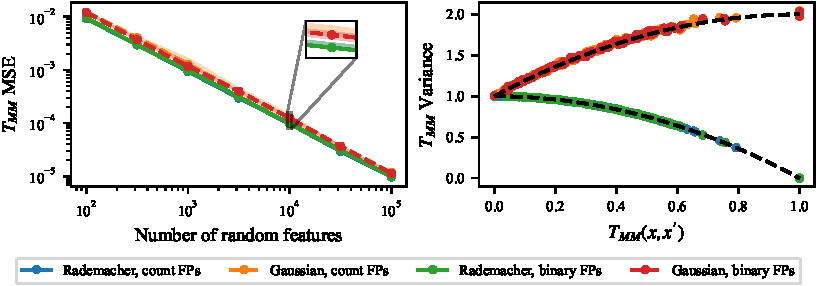
\includegraphics{chapter0x-TRF/new-figures/tmm_variance.pdf}
    \caption[Errors of TMM random features on real data]{
    \textbf{Left:} MSE of $T_{MM}$ matrix reconstruction as a function of number of random features (median over 5 trials, shaded regions are first/third quartiles).
    \textbf{Right:} empirical variance of scalar $T_{MM}$ random feature estimates for $M=10^5$,
    closely matching theoretical predictions (dashed lines).
    }
    \label{fig:tmm-rfs}
\end{figure}

Here we study the error of approximating matrices of Tanimoto coefficients using our random features,
with the general goal of verifying the claims in sections~\ref{sec:minmax-rf}--\ref{sec:t-dp} on a realistic dataset of molecules.
We choose to study a sample of 1000
small organic molecules from the GuacaMol dataset \citep{brown2019guacamol,mendez2019chembl} %
which exemplify the types of molecules typically considered in drug discovery projects.
We use both binary (B) and count (C) fingerprints of radius 2.

First, we investigate the random features for $T_{MM}$ proposed in section~\ref{sec:minmax-rf}.
We instantiate these features using the random hash from \citet{ioffe2010improved} (explained further in Appendix~\ref{apdx:explain tmm features and hash})
with $\Xi$ both Gaussian and Rademacher distributed.
The results are shown in Figure~\ref{fig:tmm-rfs}.
The left subplot shows the median mean squared error (MSE), i.e.
$$\mathbb{E}_{i,j} \left[\left(T_{MM}(x^{(i)}, x^{(j)})-\phi(x^{(i)})\cdot \phi(x^{(j)}) \right)^2\right]$$ as a function of the random feature dimension $M$.
As expected for a Monte Carlo estimator, the square error decreases with $\mathcal O(1/M)$ (i.e.\@ increasing the number of random features by 10 reduces the MSE by a factor of 10).
As predicted by Theorem~\ref{thm:general-minmax-rf},
the estimation error seems to depend only on the distribution of $\Xi$ and not on the input vectors themselves;
therefore the error curves for count and binary fingerprints overlap completely.
The error is lowest when $\Xi$ is Rademacher distributed, although the empirical difference in error seems small.
The right subplot looks at the variance across scalar random features,
showing close matching with the predictions of Theorem~\ref{thm:general-minmax-rf}.
Overall these features behave exactly as expected.

\begin{figure}
    \centering
    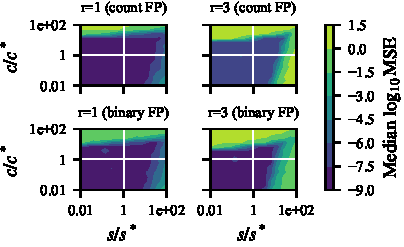
\includegraphics{chapter0x-TRF/new-figures/tdp_prefactor_contours.pdf}
    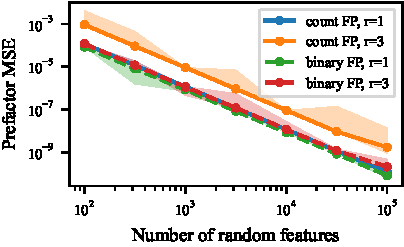
\includegraphics{chapter0x-TRF/new-figures/prefactor_mse.pdf}
    \caption[Errors of TDP prefactor random features on real data.]{
    \textbf{Left:} Contour plots of MSE for prefactor random features with $M=10^4$ with varying $s,c$.
    \textbf{Right:} MSE vs number of prefactor random features with $s,c$ values from \Cref{QMC error}.
    As in Figure~\ref{fig:tmm-rfs}, lines are medians over 5 trials, shaded regions are first/third quartiles.
    }
    \label{fig:prefactor-rfs}
\end{figure}

Next, we investigate the random features for $T_{DP}$ from section~\ref{sec:t-dp}.
These features are more complex, so we start by studying the random features for the ``prefactor''
from section~\ref{ssec:prefactor-rf}.
Recall that these features had free parameters $s,c>0$.
Fixing the number of features $M=10^4$,
Figure~\ref{fig:prefactor-rfs} (left) shows the MSE for the $r=1$ and $r=3$ terms
for both the binary and count fingerprints (which have different norms) as a function of $s$ and $c$.
The values which minimise the relative error bound from \cref{QMC error},
denoted $s^*,c^*$,
seem to lie in a broad plateau of low error in all settings,
suggesting that these values of $s,c$ are a prudent choice.
Using these values of $s,c$,
Figure~\ref{fig:prefactor-rfs} (right) shows the MSE with respect to the number of features $M$.
As expected for a QMC method,
the error dependence appears to be \emph{quadratic} $\mathcal O(1/M^2)$ (i.e.\@ a ten-fold increase in $M$ reduces MSE by 100-fold).


Because it is implemented in \texttt{scikit-learn} \citep{scikit-learn},
we use \textsc{TensorSketch} \citep{pagh2013compressed}
both as the polynomial random feature map and to combine the polynomial and prefactor
random features.
We fix the number of random features for the prefactor to be $10^4$ (recall it can be chosen freely without impacting the final random feature dimension).
Figure~\ref{fig:tdp-polynomial-and-single-term-error} shows the MSE of approximating both $(x\cdot x')^r$
and $((x\cdot x')/(\|x\|^2+\|x'\|^2))^r$.
In both cases, the MSE decreases approximately with $\mathcal O(1/M)$.
Finally, we empirically examine how to allocate $M$ random features across $R$ terms.
Using $R=4$, Figure~\ref{fig:tdp-total-rf} (left) shows that allocating most of the features to the terms with small $R$ results in lower error.
We therefore heuristically suggest allocating features according to $\tilde{m}_r\propto r^{-1}$.
Recall that truncating the power series biases the random features downward,
and in section~\ref{sec:tdp-rf} two bias correction techniques were proposed.
Figure~\ref{fig:tdp-total-rf} (right) studies the overall MSE for the plain features
and both bias correction techniques.
It appears that, in practice, neither technique is particularly helpful (normalization in fact appears harmful for large $M$).
All techniques show an error dependence of approximately $\mathcal O(1/M)$.

\begin{figure}[ht]
    \centering
    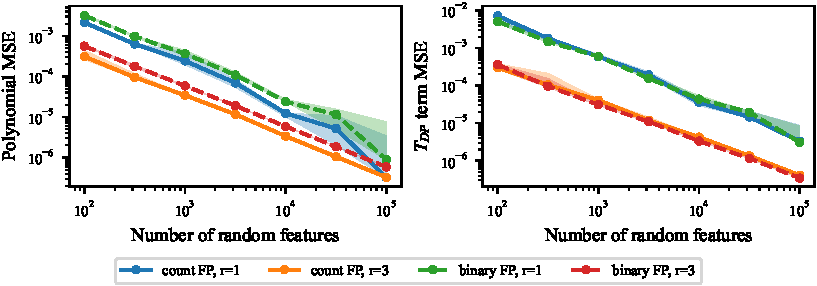
\includegraphics{chapter0x-TRF/new-figures/poly_and_term_term_mse.pdf}
    \caption[Errors of polynomial and single-term random features on real data.]{
        MSEs for approximating $(x\cdot x')^r$ (\textbf{left})
        and $((x\cdot x')/(\|x\|^2+\|x'\|^2))^r$ (\textbf{right})
        using \textsc{TensorSketch} for various $r$ on count and binary fingerprints
        as a function of the random feature dimension $M$.
    }
    \label{fig:tdp-polynomial-and-single-term-error}
\end{figure}


\begin{figure}
    \centering
    {Binary fingerprints} \\
    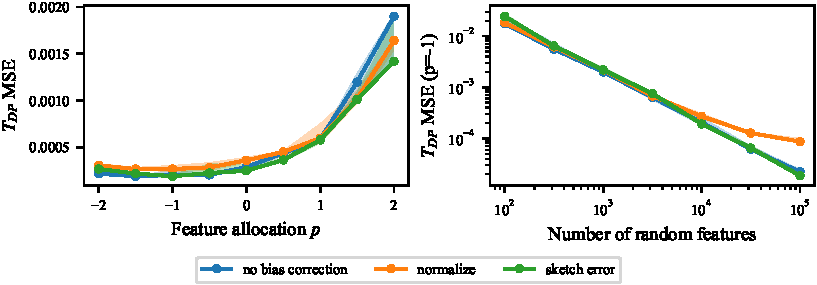
\includegraphics{chapter0x-TRF/new-figures/tdp_feat_alloc_and_overall_error_binary.pdf} \\
    {Count fingerprints}\\
    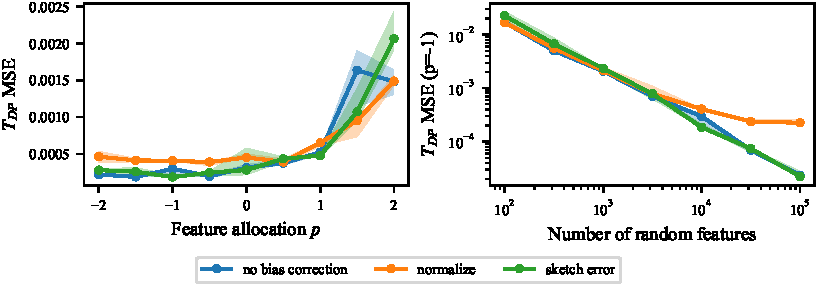
\includegraphics{chapter0x-TRF/new-figures/tdp_feat_alloc_and_overall_error_count.pdf}
    \caption[Errors of TDP random features on real data.]{
    \textbf{Left:} MSE for $M=10^4$ dimensional random features when allocating features by $\tilde{m}_r\propto r^p$, $r=1.\ldots,4$.
    \textbf{Right:}  MSE of $T_{DP}$ random features using $R=4,p=-1$ and various bias correction strategies.
    As in Figure~\ref{fig:tmm-rfs}, lines are medians over 5 trials, shaded regions are first/third quartiles.
    }
    \label{fig:tdp-total-rf}
\end{figure}




\subsection{Molecular property prediction and uncertainty quantification}\label{sec:regression-expt}

To evaluate their efficacy in practice, we use our random features to approximate large-scale Gaussian processes (GPs) \citep{rasmussen2006gp}
for molecular property prediction.
Specifically, we study 5 tasks from the \textsc{dockstring} benchmark 
which entail predicting protein binding affinity from a molecular graph structure \citep{ortegon2021dockstring}.
Each task contains $250\mathrm{k}$ molecules, making exact GP regression infeasible. 
We represent molecules with count Morgan fingerprints of radius 1.

We use $M=5000$ random features for all methods.
We compare to two approximate GP baselines.
The first is an exact GP on a random subset of size $M$.
Since this approach ignores most of the dataset,
one should expect a reasonable approximate GP to perform better.
The second is a sparse variational GP (SVGP) which approximates the dataset using $M$ pseudo-data points $Z$
\citep{titsias2009variational,hensman2013gaussian}.
The locations of $Z$ are typically chosen based on the input dataset (we use K-means clustering),
making this method effectively a data-dependent sketch.
Accordingly, one might expect the performance of this approximation to be \emph{better}
than data-oblivious random features.
Details of Gaussian process training are given in \cref{apdx:regression-expt-details}.

\begin{table*}[tb]
\caption[Average log probabilities of dockstring test set labels with various approximate GPs.]{
Average log probability of test set labels with various approximate GPs
for 5 targets from \textsc{dockstring} dataset \citep{ortegon2021dockstring}.
$\pm$ values are standard deviations over 5 trials.
}
\label{tab:gp-regression-logp}
\begin{center}
\resizebox{0.95\textwidth}{!}{
\begin{sc}
\begin{tabular}
{llr@{\hspace{0.02cm}$\pm$\hspace{0.02cm}}l@{\hspace{0.30cm}}r@{\hspace{0.02cm}$\pm$\hspace{0.02cm}}l@{\hspace{0.30cm}}r@{\hspace{0.02cm}$\pm$\hspace{0.02cm}}l@{\hspace{0.30cm}}r@{\hspace{0.02cm}$\pm$\hspace{0.02cm}}l@{\hspace{0.30cm}}r@{\hspace{0.02cm}$\pm$\hspace{0.02cm}}l@{\hspace{0.30cm}}}
\toprule
Kernel & Method & \multicolumn{2}{c}{ESR2} & \multicolumn{2}{c}{F2} & \multicolumn{2}{c}{KIT} & \multicolumn{2}{c}{PARP1} & \multicolumn{2}{c}{PGR}\\
\midrule
$T_{MM}$ & Rand subset GP & -1.084 & 0.004 & -0.951 & 0.002 & -1.094 & 0.002 & -0.999 & 0.002 & -1.183 & 0.005\\
 & SVGP & -0.908 & 0.005 & -0.502 & 0.005 & -0.846 & 0.002 & -0.606 & 0.005 & -1.030 & 0.005\\
 & RFGP ($\Xi$ Rad.) & -0.954 & 0.009 & -0.658 & 0.013 & -1.222 & 0.044 & -0.968 & 0.037 & -1.127 & 0.023\\
 & RFGP ($\Xi$ Gauss.) & -0.956 & 0.010 & -0.663 & 0.015 & -1.230 & 0.048 & -0.967 & 0.036 & -1.124 & 0.025\\
\midrule
$T_{DP}$ & Rand subset GP & -1.073 & 0.002 & -0.940 & 0.001 & -1.077 & 0.002 & -0.988 & 0.001 & -1.187 & 0.006\\
 & SVGP & -0.880 & 0.004 & -0.459 & 0.002 & -0.804 & 0.002 & -0.568 & 0.002 & -1.010 & 0.004\\
 & RFGP (plain) & -0.902 & 0.003 & -0.513 & 0.004 & -0.979 & 0.015 & -0.690 & 0.022 & -1.029 & 0.002\\
 & RFGP (norm) & -0.902 & 0.003 & -0.515 & 0.003 & -0.980 & 0.015 & -0.691 & 0.022 & -1.028 & 0.002\\
 & RFGP (sketch) & -0.904 & 0.002 & -0.515 & 0.004 & -0.979 & 0.014 & -0.690 & 0.021 & -1.030 & 0.002\\
\bottomrule
\end{tabular}

\end{sc}
}
\end{center}
\end{table*}

Table~\ref{tab:gp-regression-logp} shows the average log probability\footnote{
    Calculated by first calculating the log probability of each test point individually
    (i.e.\@ marginally, not jointly), then averaging these values.
}
of test set labels
for all types of GP with $T_{MM}$ and $T_{DP}$ kernels.
Several trends are evident.
First, for each kernel random feature GPs (RFGPs) consistently outperform random subset GPs,
but underperform SVGP.
Second, for each kernel the difference between the RFGP varieties is small
(generally less than the standard deviation).
Third, on most targets $T_{DP}$ seems to perform better than the $T_{MM}$ kernel.
The reason for this is unclear.

Similar trends can be seen in the $R^2$ metric\footnote{
    This is calculated using the function \texttt{sklearn.metrics.r2\_score}.
    This measures only the error of the GP mean.
    A value of 1 indicates perfect prediction,
    while a value of 0 can be achieved by predicting the sample mean for every data point.
}
in Table~\ref{tab:gp-regression-r2}.
Because $R^2$ only uses point predictions,
we also include baselines for two types of graph neural network:
Attentive FP \citep{xiong2019pushing}
and MPNN \citep{gilmer2017neural}.
Although the performance of GP methods does not match that of Attentive FP,
it is often close,
suggesting there is potential for approximate GPs to be competitive with graph neural networks
for molecular property prediction.

Overall, this suggests that the RFGPs developed in this chapter can be used in large-scale regression,
although it seems in practice that data-dependent approximations are more accurate.

\begin{table*}[tb]
\caption[$R^2$ scores of various approximate GPs on dockstring test set.]{
Average $R^2$ score for approximate GPs on \textsc{dockstring} dataset.
Attentive FP and MPNN results
are taken from \citet{ortegon2021dockstring}.
Other details are the same as Table~\ref{tab:gp-regression-logp}.
}
\label{tab:gp-regression-r2}
\begin{center}
\resizebox{0.95\textwidth}{!}{
\begin{sc}
\begin{tabular}
{llr@{\hspace{0.02cm}$\pm$\hspace{0.02cm}}l@{\hspace{0.30cm}}r@{\hspace{0.02cm}$\pm$\hspace{0.02cm}}l@{\hspace{0.30cm}}r@{\hspace{0.02cm}$\pm$\hspace{0.02cm}}l@{\hspace{0.30cm}}r@{\hspace{0.02cm}$\pm$\hspace{0.02cm}}l@{\hspace{0.30cm}}r@{\hspace{0.02cm}$\pm$\hspace{0.02cm}}l@{\hspace{0.30cm}}}
\toprule
Kernel & Method & \multicolumn{2}{c}{ESR2} & \multicolumn{2}{c}{F2} & \multicolumn{2}{c}{KIT} & \multicolumn{2}{c}{PARP1} & \multicolumn{2}{c}{PGR}\\
\midrule
$T_{MM}$ & Rand subset GP & 0.514 & 0.002 & 0.810 & 0.002 & 0.695 & 0.002 & 0.849 & 0.001 & 0.426 & 0.007\\
 & SVGP & 0.578 & 0.001 & 0.861 & 0.000 & 0.749 & 0.000 & 0.889 & 0.000 & 0.542 & 0.002\\
 & RFGP ($\Xi$ Rad.) & 0.518 & 0.002 & 0.838 & 0.001 & 0.703 & 0.002 & 0.864 & 0.001 & 0.465 & 0.003\\
 & RFGP ($\Xi$ Gauss.) & 0.517 & 0.002 & 0.837 & 0.000 & 0.702 & 0.001 & 0.864 & 0.001 & 0.467 & 0.004\\
\midrule
$T_{DP}$ & Rand subset GP & 0.513 & 0.003 & 0.817 & 0.001 & 0.696 & 0.002 & 0.851 & 0.001 & 0.384 & 0.011\\
 & SVGP & 0.581 & 0.001 & 0.865 & 0.000 & 0.753 & 0.001 & 0.889 & 0.000 & 0.543 & 0.002\\
 & RFGP (plain) & 0.546 & 0.001 & 0.852 & 0.001 & 0.716 & 0.002 & 0.876 & 0.000 & 0.512 & 0.002\\
 & RFGP (norm) & 0.546 & 0.001 & 0.852 & 0.001 & 0.715 & 0.002 & 0.876 & 0.000 & 0.513 & 0.002\\
 & RFGP (sketch) & 0.545 & 0.001 & 0.852 & 0.001 & 0.716 & 0.002 & 0.876 & 0.000 & 0.510 & 0.002\\
\midrule
N/A & MPNN & 0.506 & 0.001  & 0.798 & 0.005  & 0.755 & 0.005  & 0.815 &  0.010 & 0.324 &  0.096 \\
N/A & Attentive FP & 0.627 &  0.010 & 0.880 &  0.001 & 0.806 &  0.008 & 0.910 &  0.002 & 0.678 & 0.008 \\
\bottomrule
\end{tabular}

\end{sc}
}
\end{center}
\end{table*}





\subsection{Bayesian optimisation in molecule space via Thompson sampling}\label{sec:expt-bayesopt}

Bayesian optimisation (BO) uses a probabilistic surrogate model to guide optimisation
and is generally considered one of the most promising techniques for sample-efficient optimisation \citep{shahriari2015taking}.
Because wet-lab experiments are expensive and time-consuming,
there is considerable interest in using BO for experiment design.
Chemistry experiments are often done in large batches,
and therefore algorithms which use functions sampled from a probabilistic model are of particular interest \citep{hernandez2017parallel}.
To sample from a normal distribution $\mathcal{N}(\mu,K)$ one typically transforms i.i.d.\@ samples $Z~\sim\mathcal{N}(0,1)$ via $\mu+K^{1/2}Z$.
This requires computing $K^{1/2}$, and thereby causes exact GP sampling to scale cubically in the number of \emph{evaluation} points.
By approximating $K\approx \Phi^T \Phi$,
our random features allow for approximate sampling in \emph{linear} time.
In this section we apply this to a real-world dataset.

\begin{figure}[h]
    \centering
    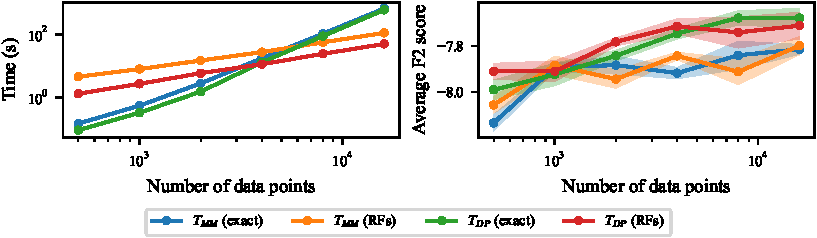
\includegraphics{chapter0x-TRF/new-figures/bo_results.pdf}
    \caption[Results of Bayesian optimisation using exact and approximate Thompson sampling.]{
        Run time and docking scores of BO using exact and approximate Thompson sampling.
        Solid lines are means over 5 trials, shaded regions are standard errors.
    }
    \label{fig:thompson-sampling-results}
\end{figure}

As a demonstration, we consider a single round of selecting 100 molecules from a random sub-sample of $n$ molecules using \emph{Thompson sampling}
(equation~\ref{eqn:backgroun:thompson sampling}) with the $T_{MM}$ and $T_{DP}$ kernels.
Similar to the setup from section~\ref{sec:regression-expt},
we use molecules and labels from the \textsc{dockstring} dataset.
Molecules are represented as count fingerprints.
$M=5000$ random features used, with Rademacher $\Xi$ for $T_{MM}$ and no bias correction for $T_{DP}$.
All other implementation details are the same as in the previous subsection.
Figure~\ref{fig:thompson-sampling-results} (left) shows that,
as expected, exact Thompson sampling scales worse than
approximate Thompson sampling with random features.
Figure~\ref{fig:thompson-sampling-results} (right) shows that using approximate instead of exact Thompson sampling does not seem to change the average F2 docking scores of the molecules chosen.
This suggests that approximate Thompson sampling could fruitfully be applied to large datasets of molecules
in Bayesian optimisation tasks.
